\section{Raka mottagare}
\textbf{HAREC a.\ref{HAREC.a.4.1.2}\label{myHAREC.a.4.1.2}}
\index{rak mottagare}
\index{mottagare!rak}

\subsection{Mottagare med kristalldetektor}
\index{kristalldetektor}
\index{mottagare!kristal}

\begin{figure}
  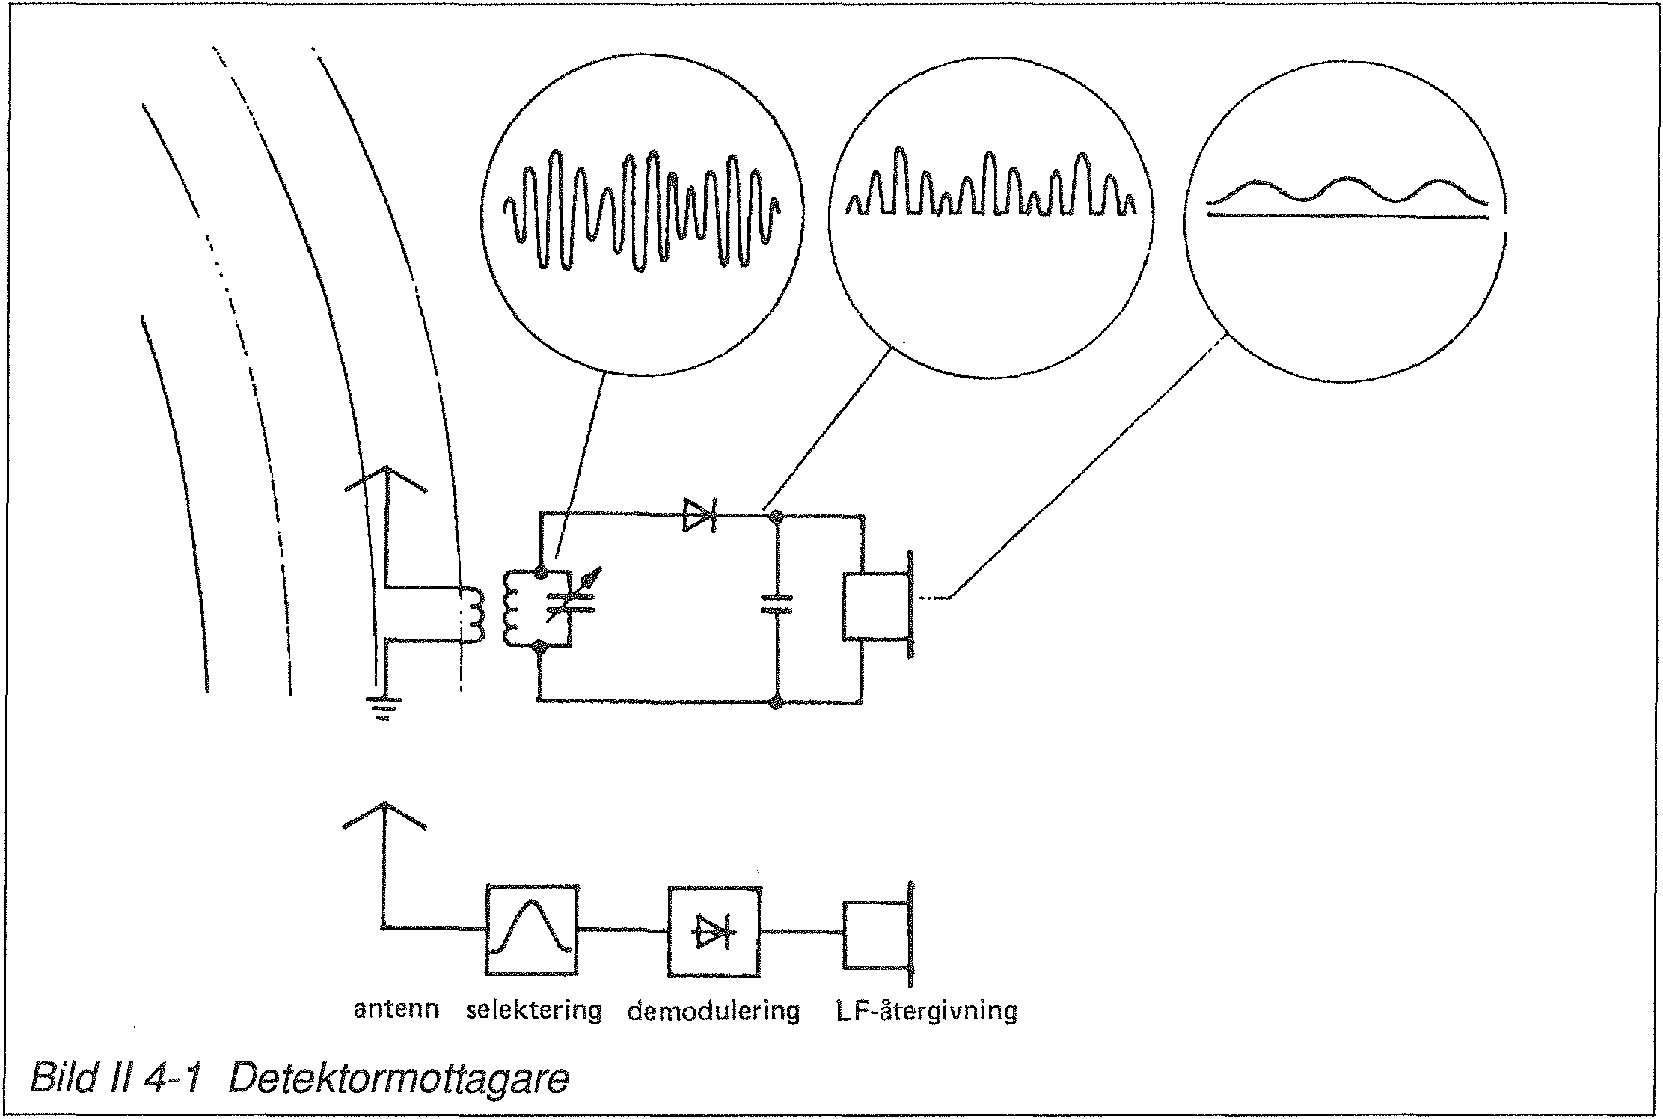
\includegraphics[width=\textwidth]{images/bild_2_4-01}
  \caption{Detektormottagare}
  \label{fig:bildII4-1}
\end{figure}

Bild \ref{fig:bildII4-1}

Detektormottagaren består av ett mycket litet antal
komponenter. Princip och arbetssätt framgår av bilden. Samma princip
används även i mer komplicerade mottagare, mätinstrument
etc. Antennkretsen består av antenn, jordtag och däremellan en
induktor (kopplingsspole), som överför energin från antennen till en
svängningskrets. Svängningskretsen används för att välja ut (selektera)
en bärvåg med önskad frekvens. Bärvågen kan naturligtvis inte
höras, men av kurvformen på bilden framgår att bärvågen är
amplitudmodulerad med en LF-signal.

För att återvinna LF-signalen utför man en s.k. demodulering med hjälp
av dioden.  Dioden klipper bort antingen de positiva eller negativa
halvvågorna i den mottagna signalen, beroende på hur dioden är
vändpolariserad. Kondensatorn, som är kopplad parallellt över
hörtelefonen, glättar de högfrekventa spänningstopparna till ett
amplitudmedelvärde (jämför med entaktsblandare i Kapitel 3). Detta
spänningsvärde varierar på ett sätt, som motsvarar den modulerande
spänning i sändaren som kommer av tal, musik etc. Vi har nu
demodulerat bärvågen, återställt LF-signalen och kan höra den i
mottagaren.

\begin{wrapfigure}{R}{0.5\textwidth}
  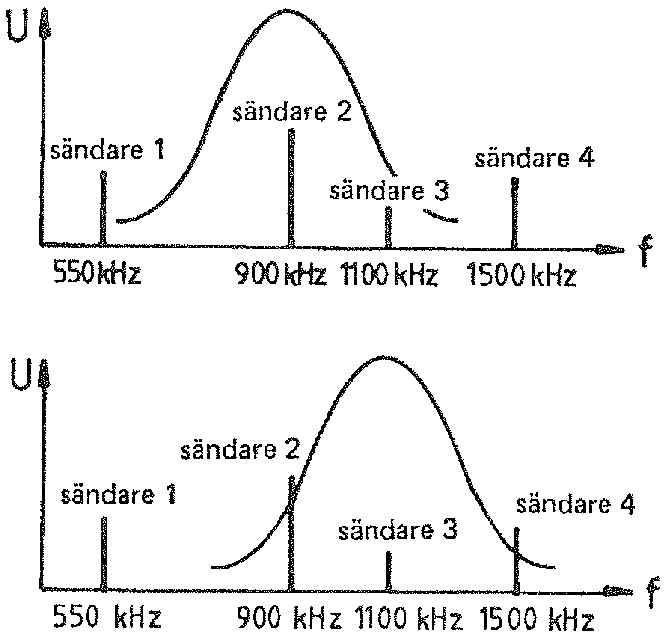
\includegraphics[width=0.5\textwidth]{images/bild_2_4-02}
  \caption{Selektion i detektormottagare}
  \label{fig:bildII4-2}
\end{wrapfigure}

Bild \ref{fig:bildII4-2}

Signalspänningen över svängningskretsen är störst när dess
resonansfrekvens och antennströmmens frekvens är lika.

Överst i bilden ser man att mottagaren är inställd på samma frekvens
som sändare 2.  Även sändare 3 hörs eftersom bandbredden i
svängningskretsen är stor. Nederst i bilden är svängningskretsen
inställd på sändare 3, men man hör också sändare 2 och 4.

Bandbredden i svängningskretsen blir mindre ju mindre den belastas,
d.v.s dämpas. I Bild \ref{fig:bildII4-1} består belastningen av antennen (via
kopplingsspolen), hörtelefonen och avkopplingskondensatorn (via
dioden).

Mindre belastning kan åstadkommas på två sätt; dels med ''lösare''
koppling mellan antennkrets och svängningskrets och dels med bättre
impedansanpassning mellan svängningskrets och diod. Båda sätten
tillämpas i Bild \ref{fig:bildII4-3}. Hur selektionen då förbättras visas i
Bild \ref{fig:bildII4-4}, vilket ska jämföras med Bild \ref{fig:bildII4-2}.

\begin{figure}
  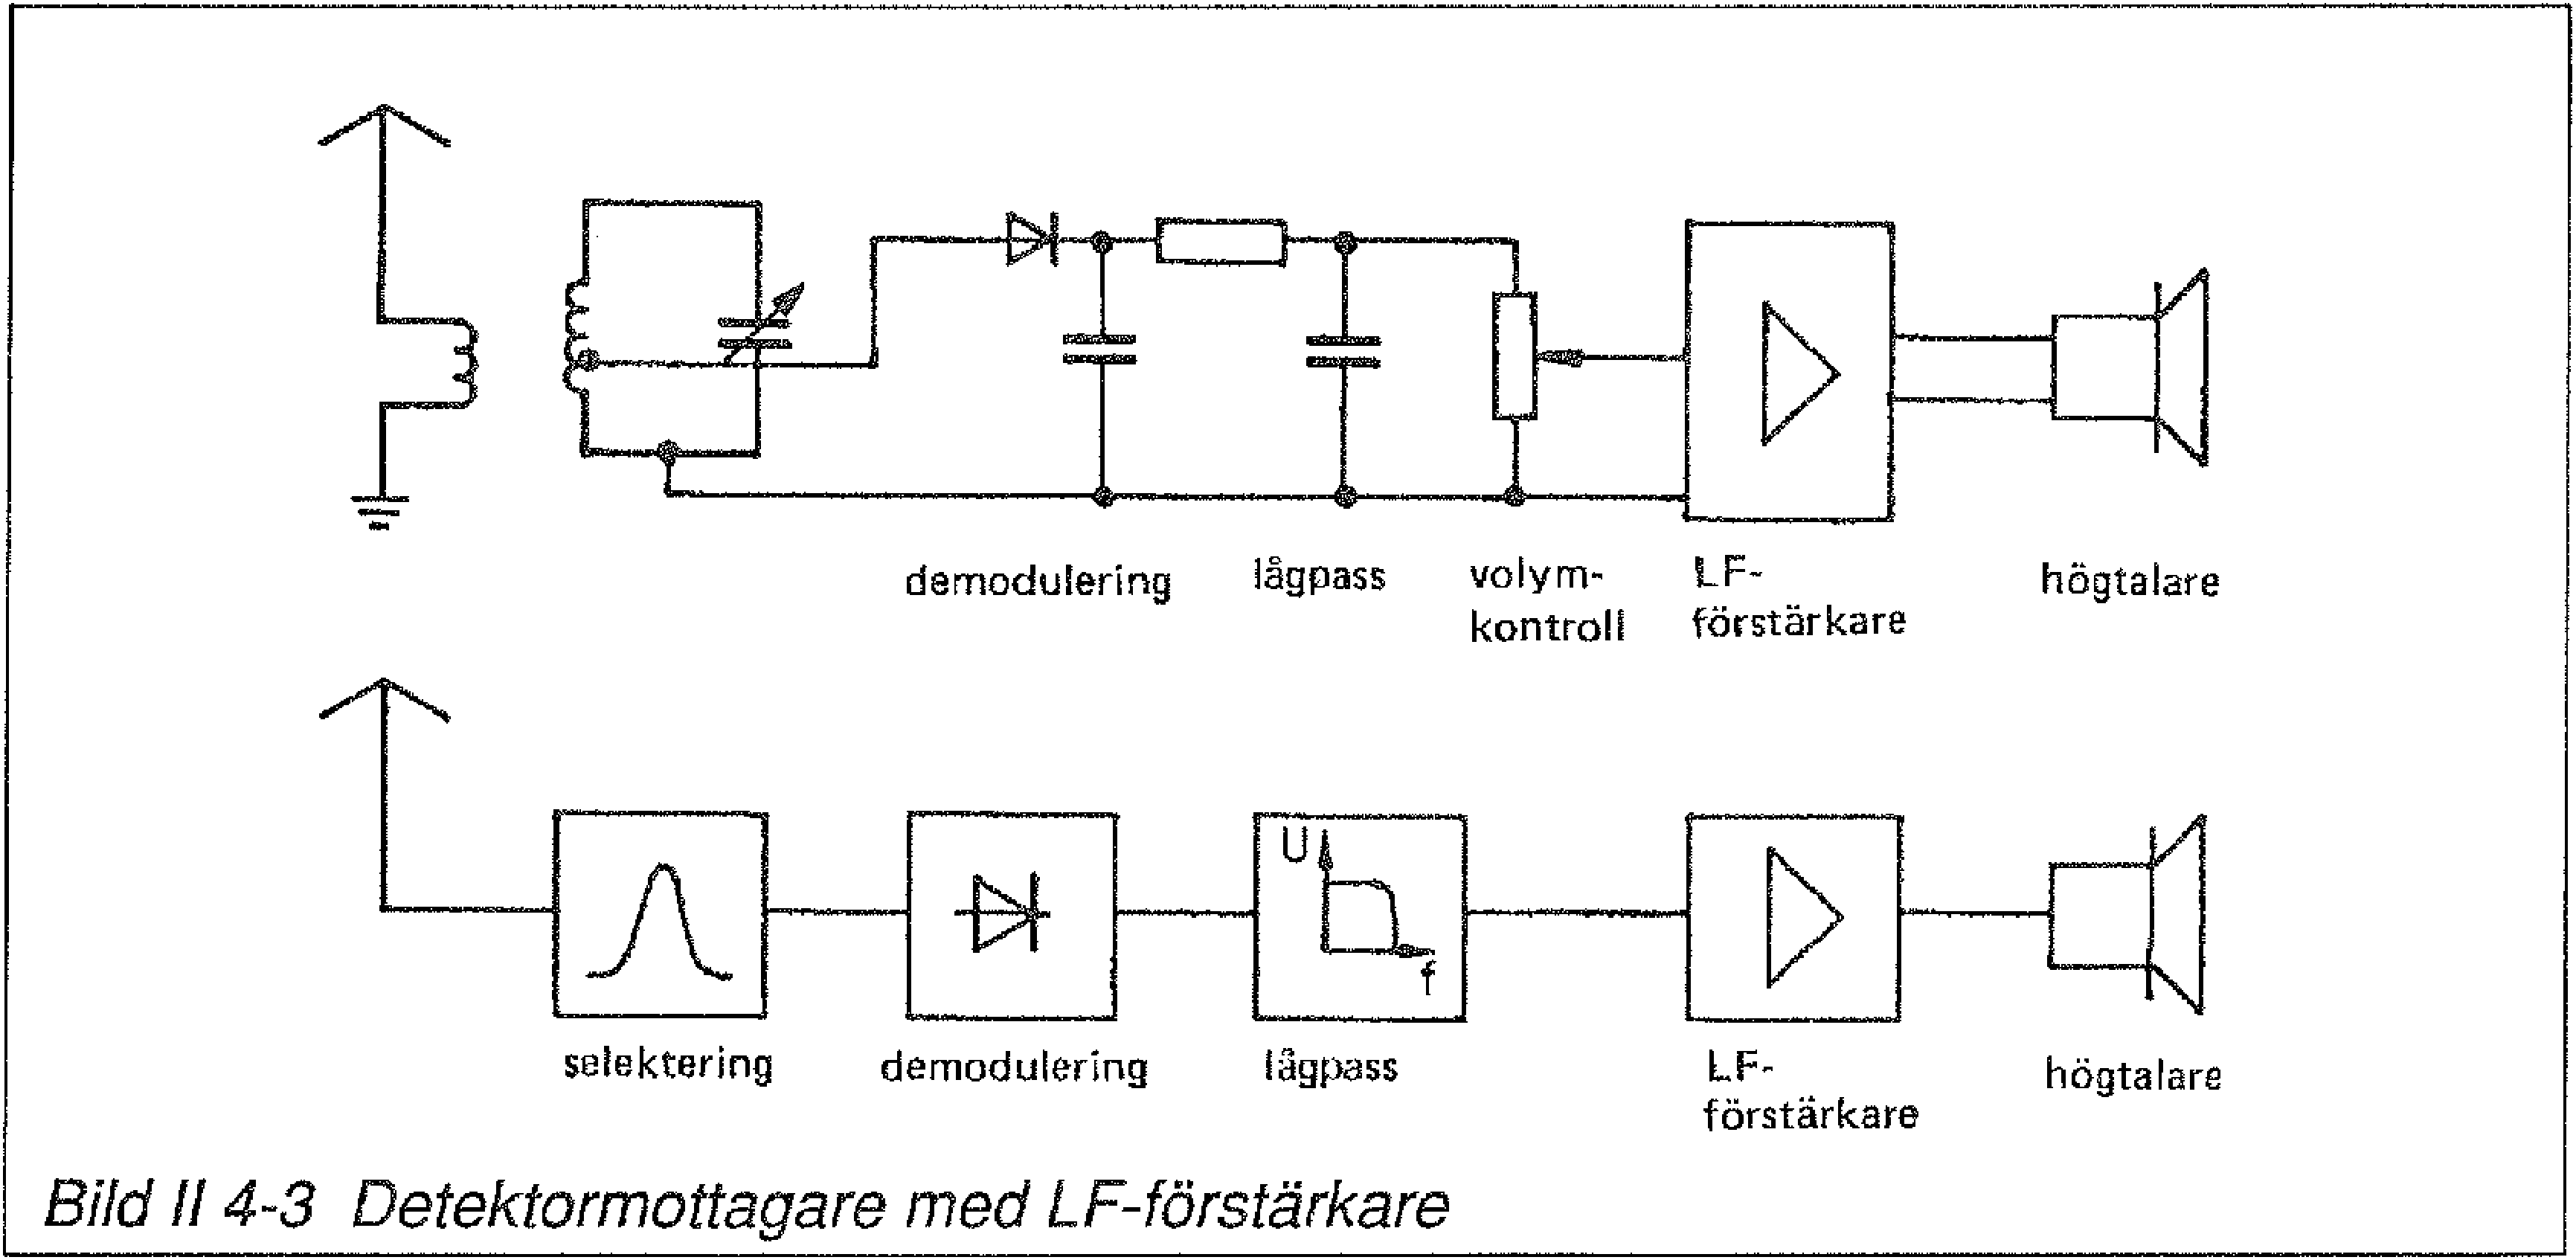
\includegraphics[width=\textwidth]{images/bild_2_4-03}
  \caption{Detektormottagare med LF-förstärkare}
  \label{fig:bildII4-3}

  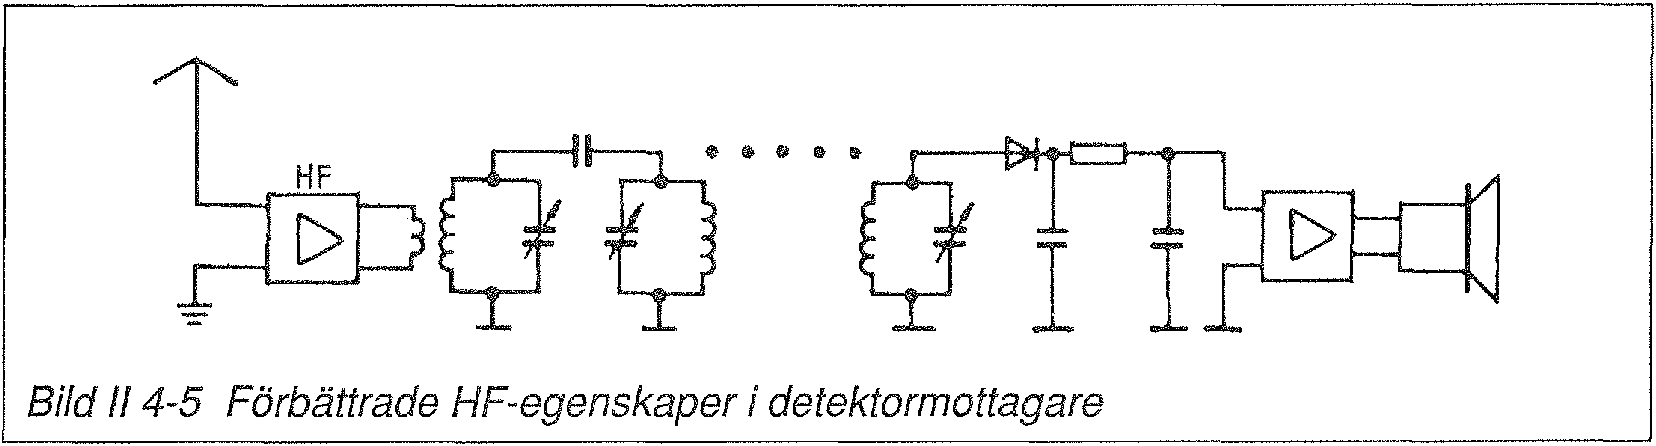
\includegraphics[width=\textwidth]{images/bild_2_4-05}
  \caption{Förbättrade HF-egenskaper i detektormottagare}
  \label{fig:bildII4-5}
\end{figure}

\subsection{Detektormottagare med förstärkare}

Bild \ref{fig:bildII4-3}

Om man vill höra sändningarna över högtalare, behövs högre effekt än
vad som kan fångas upp genom antennen. För ändamålet används en
LF-förstärkare, som drivs av en annan energikälla, t. ex. ett
batteri. LF-förstärkaren kan även minska belastningen på
svängningskretsen.

I bilden har ett LF-lågpassfilter satts in efter
HF-avkopplingskondensatorn. Det dämpar LF-signaler med högre frekvens
än vad som behövs för god mottagning.

\subsubsection{Mottagare med bättre HF-egenskaper}

Bild \ref{fig:bildII4-5}

Ett sätt att minska bandbredden i en detektormottagare är att koppla
flera svängningskretsar med samma frekvens efter varandra. Den större
dämpningen av fler kretsar kan kompenseras med en HF-förstärkare.

Sådana mottagare används för speciella ändamål, t.ex. för övervakning
av en enda frekvens. Då är svängningskretsarna fast avstämda. Kanske
utnyttjas till och med en kvartskristall som filter för den speciella
frekvensen. Se Bild \ref{fig:bildII4-6} om hög selektion.

\begin{wrapfigure}{R}{0.5\textwidth}
  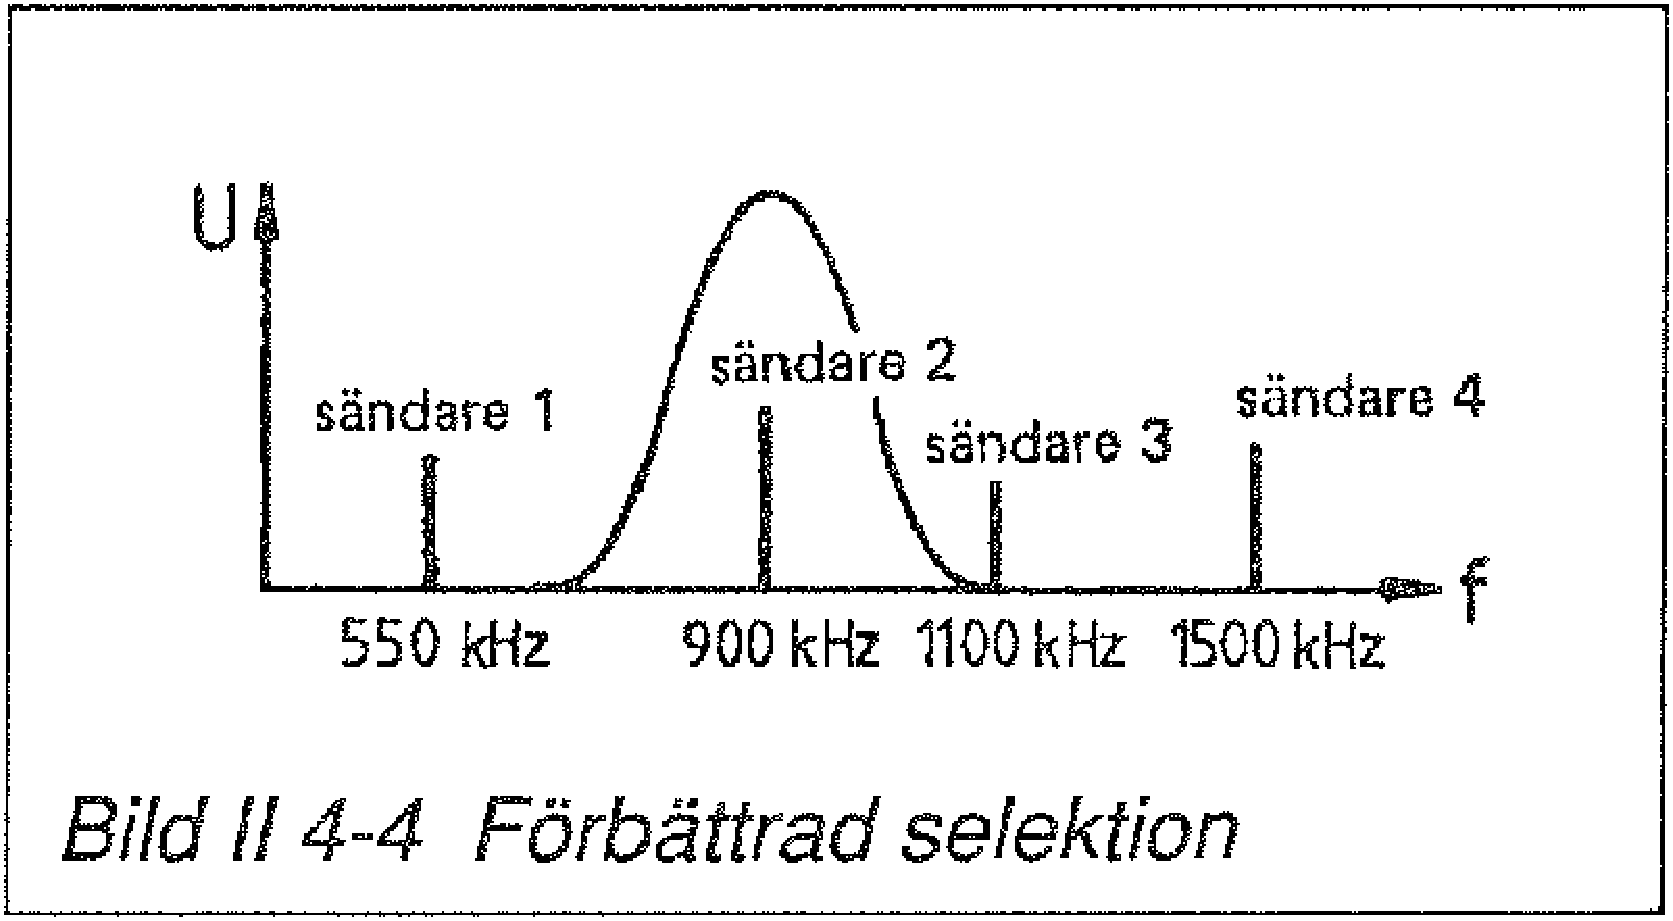
\includegraphics[width=0.5\textwidth]{images/bild_2_4-04}
  \caption{Förbättrad selektion}
  \label{fig:bildII4-4}

  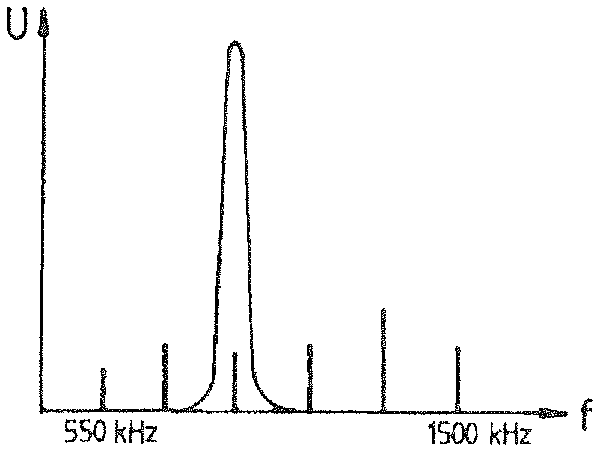
\includegraphics[width=0.5\textwidth]{images/bild_2_4-06}
  \caption{Hög HF-selektion}
  \label{fig:bildII4-6}

  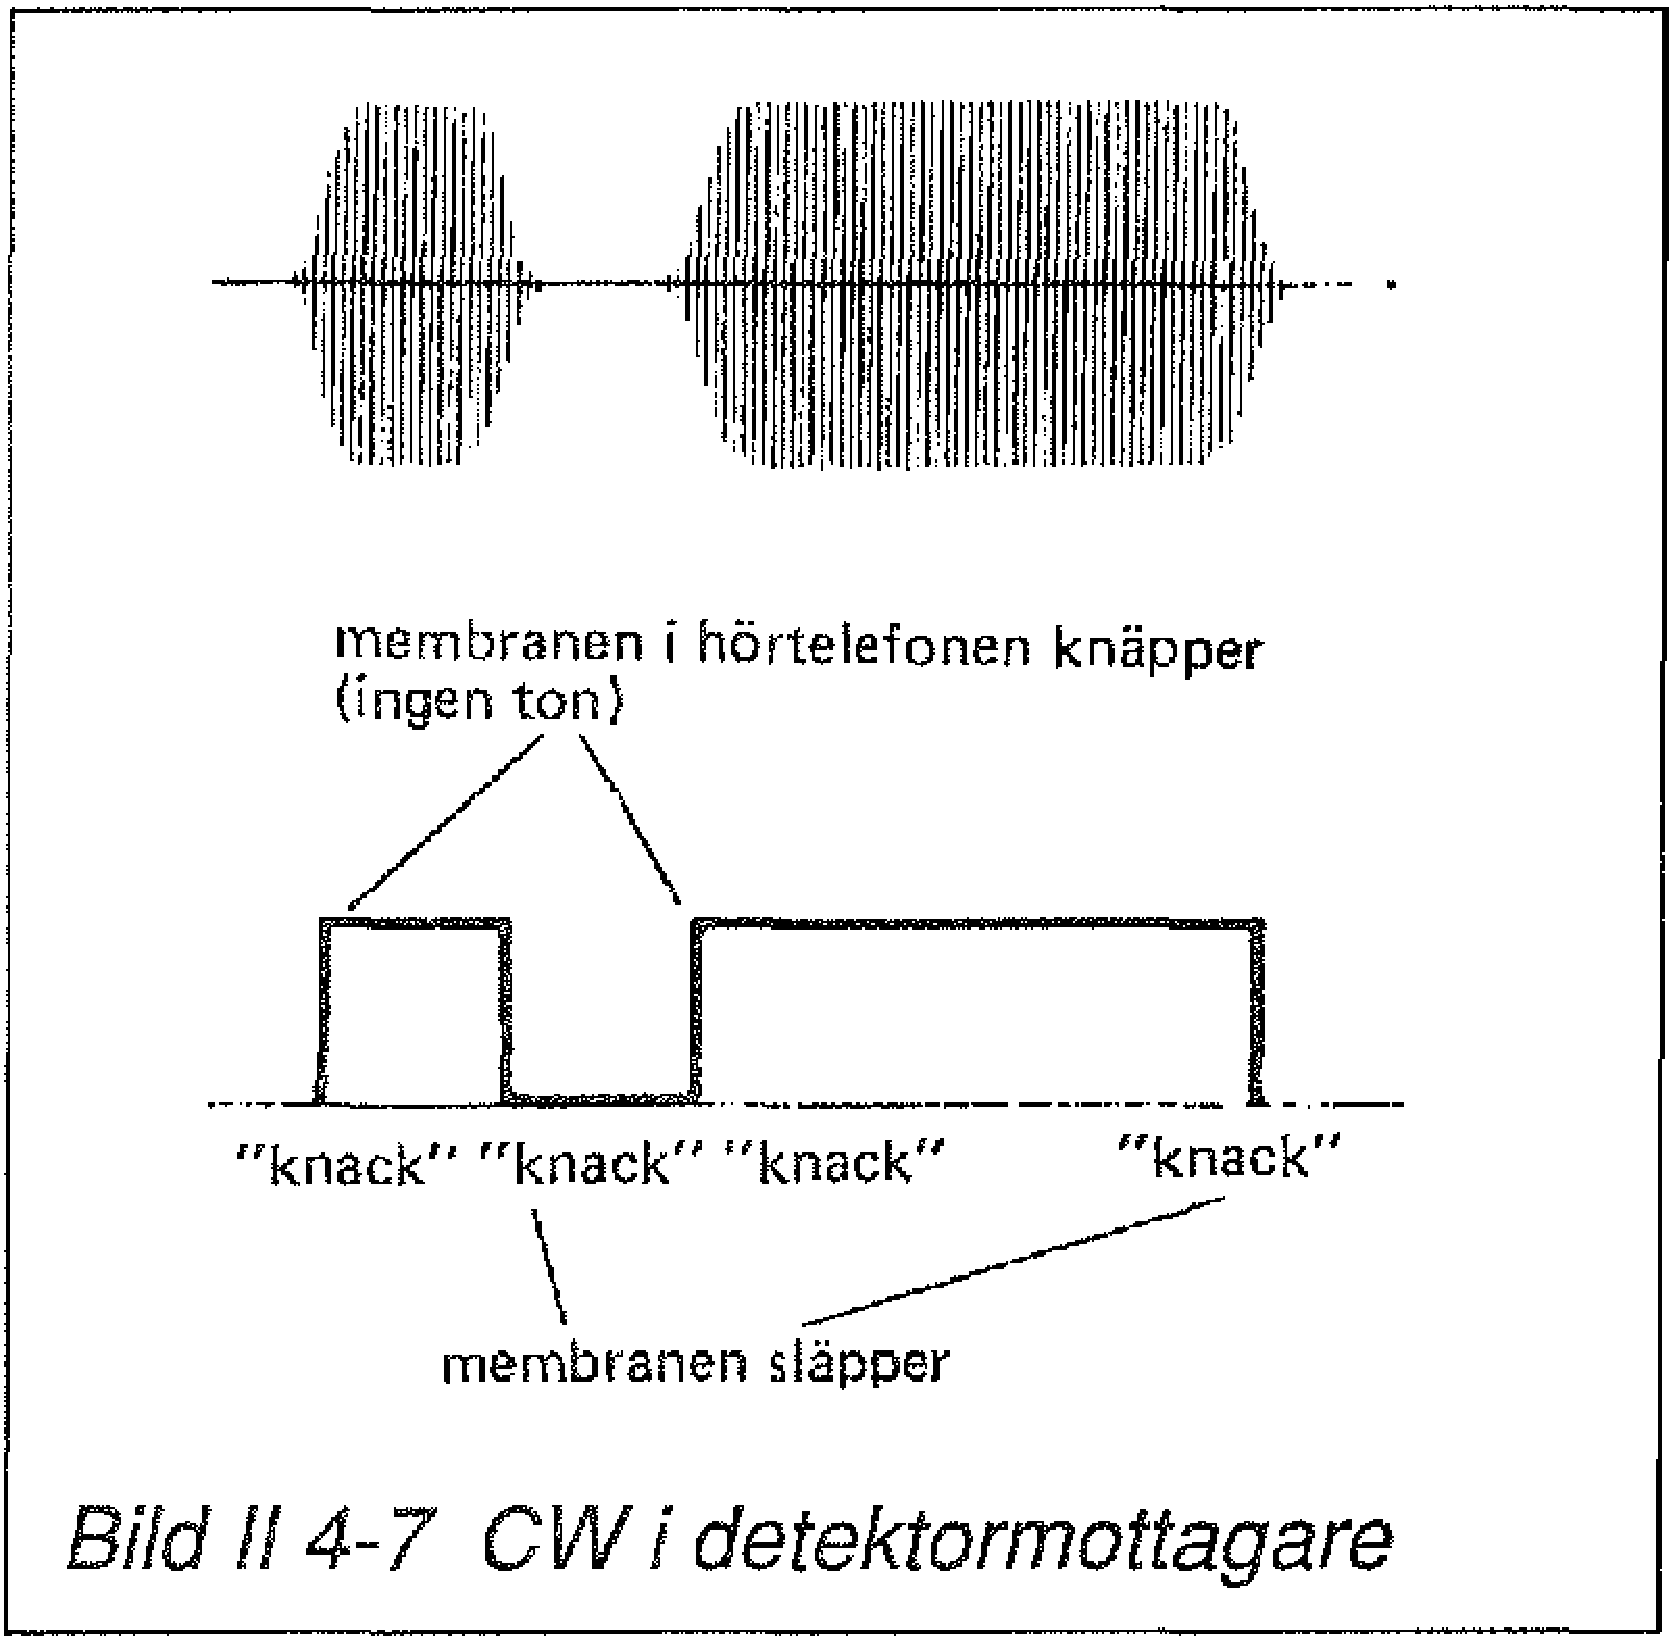
\includegraphics[width=0.5\textwidth]{images/bild_2_4-07}
  \caption{CW i detektormottagare}
  \label{fig:bildII4-7}
\end{wrapfigure}

\subsection{Detektormottagare och sändningsslag}

I huvudsak fungerar detektormottagaren endast vid
amplitudmodulering. Det innebär sändningsslagen A3E och A2A,
d.v.s. amplitudmodulerad telefoni resp. tonmodulerad telegrafi, båda
med full bärvåg.

Bild \ref{fig:bildII4-7}

Däremot fungerar detektormottagaren inte vid A1A, d.v.s. telegrafi med
endast bärvåg. En omodulerad bärvåg alstrar nämligen endast en
likström i en detektormottagare. Vid nyckling hörs då endast
knäppningar i hörtelefonen vid början och slutet av teckendelarna.

Detektormottagaren fungerar inte heller vid J3E, d.v.s. SSB och övriga
sändningsslag med undertryckt bärvåg. Ljud såsom tal förvrängs
nämligen kraftigt i en J3E-signal eftersom bärvågskomponenten saknas.

I båda ovannämnda fall kan talet återställas med tillsats av en bärvåg.
Slutligen kan sändningsslag som innebär frekvens- och fasmodulering i
princip inte demoduleras med detektormottagare.

\subsection{Mottagare med direkt frekvensblandning}
\textbf{HAREC a.\ref{HAREC.a.4.2.2}\label{myHAREC.a.4.2.2},
a.\ref{HAREC.a.4.3.2}\label{myHAREC.a.4.3.2},
a.\ref{HAREC.a.4.3.3}\label{myHAREC.a.4.3.3},
a.\ref{HAREC.a.4.3.6}\label{myHAREC.a.4.3.6},
a.\ref{HAREC.a.4.3.7}\label{myHAREC.a.4.3.7}
}
\index{frekvensblandning}
\index{mottagare!direkt frekvensblandare}

\begin{figure}
  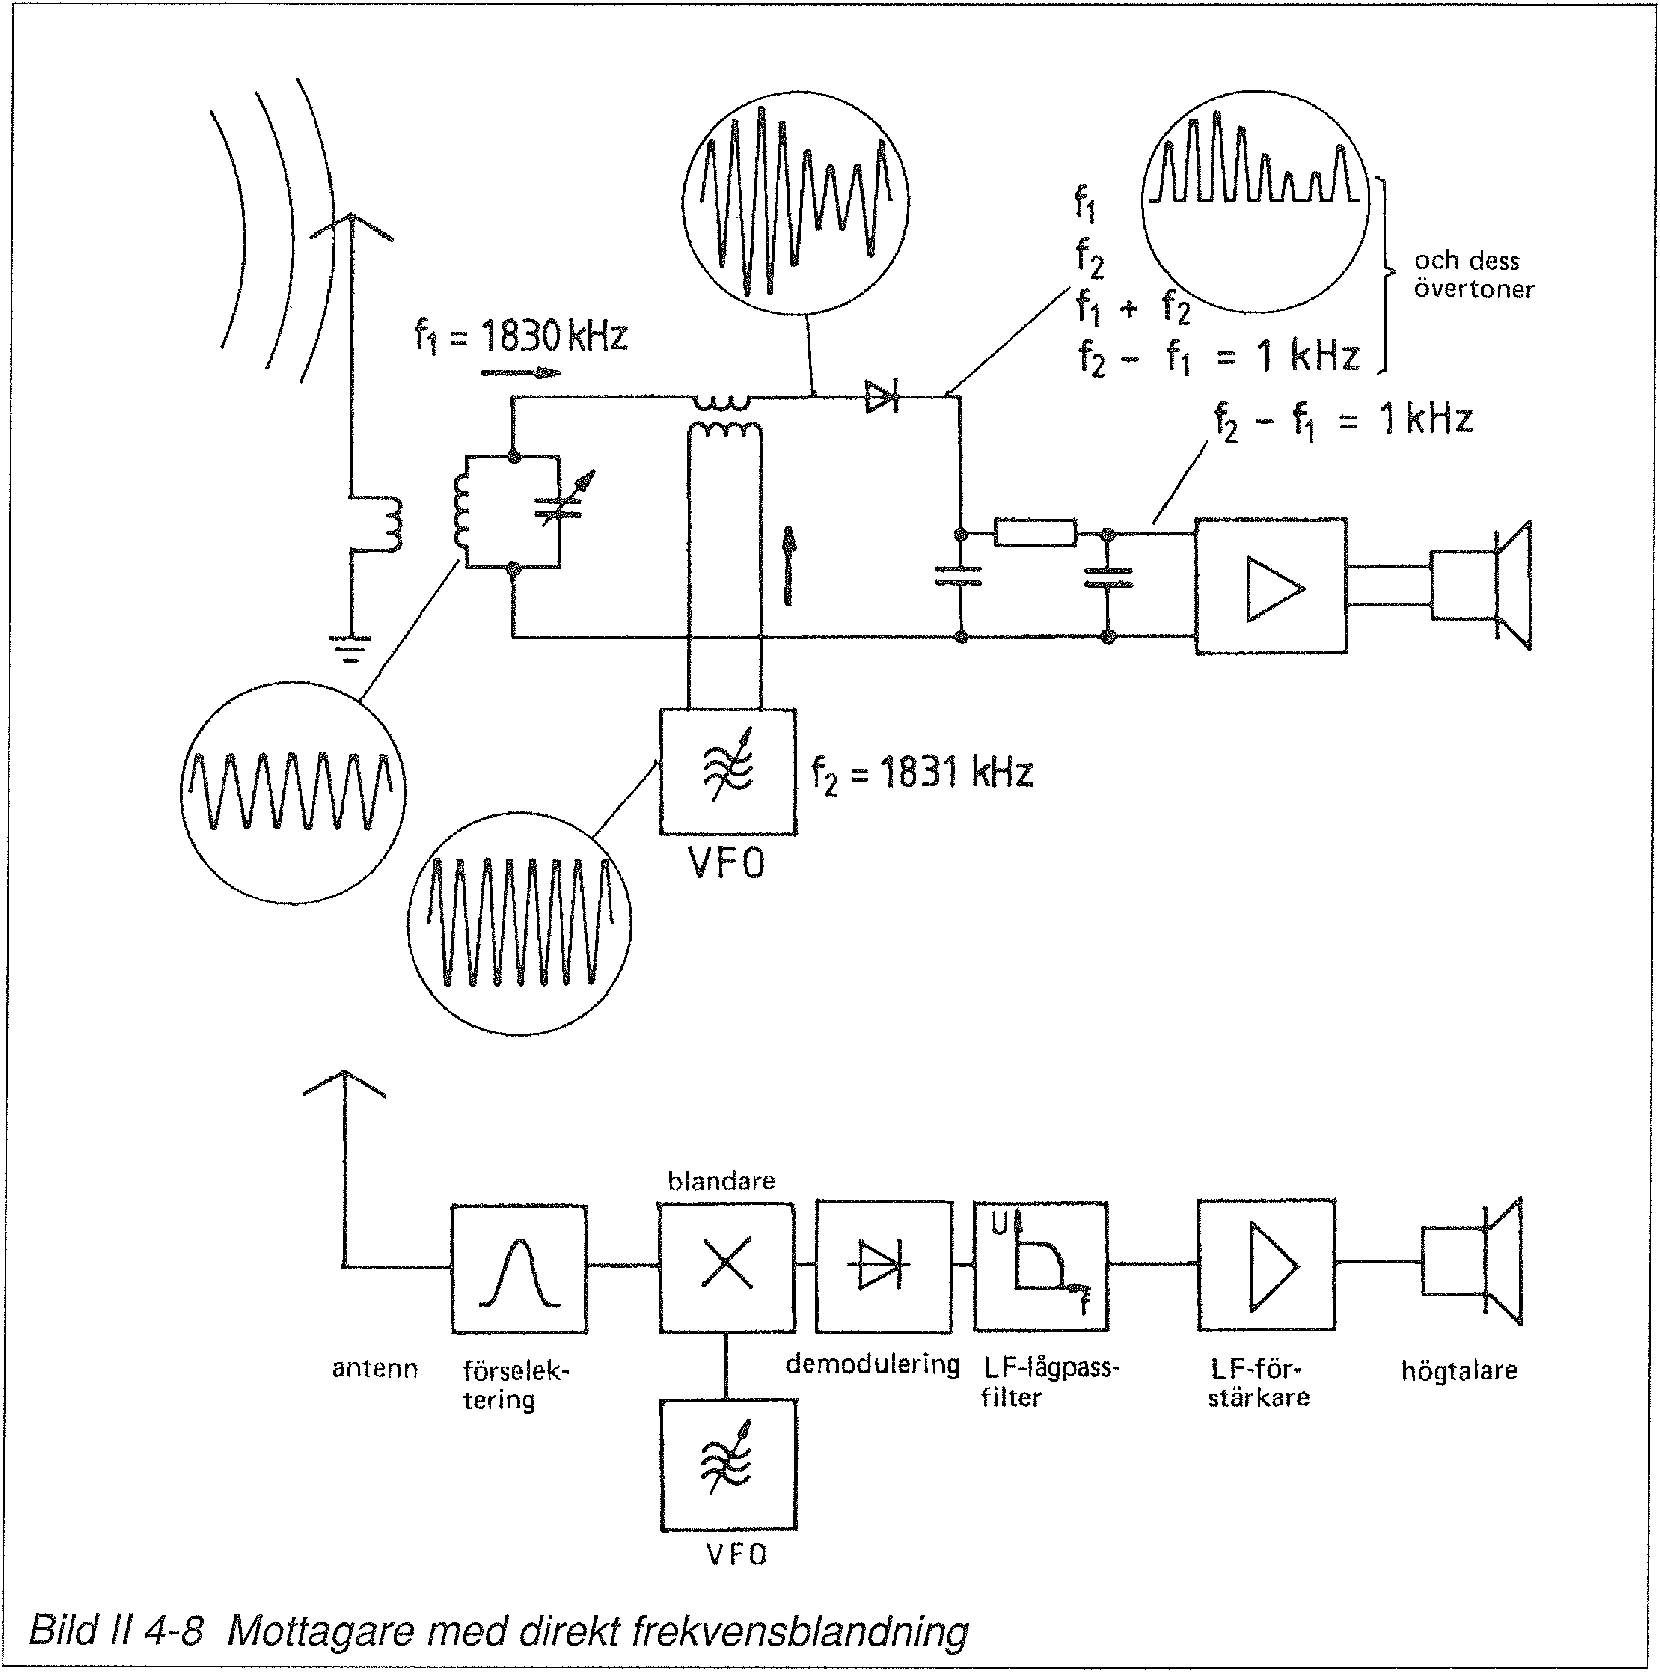
\includegraphics[width=\textwidth]{images/bild_2_4-08}
  \caption{Mottagare med direkt frekvensblandning}
  \label{fig:bildII4-8}
\end{figure}

För att demodulera A1A och J3E i en rak mottagare-
detektormottagare måste den kompletteras med en oscillator som alstrar
en intern bärvåg. Denna blandas med den mottagna signalen. Det uppstår
då en svävningston - beat frequency. Därav namnet Beat Frequency
Oscillator - BFO.

Förfarandet har givit mottagartypen sitt namn - direktblandad
mottagare.

Bild \ref{fig:bildII4-8}

Ett sätt att komplettera den raka mottagaren med BFO framgår av
bilden. När BFO kopplas till och ställs in på en frekvens tillräckligt
nära mottagningsfrekvensen så uppstår en hörbar ton.

Demodulatordioden tillförs alltså två HF-signaler, dels den från
antennen och dels den från BFO. Dessa båda signaler blandas i dioden
och skillnadsfrekvensen är den hörbara tonen. Övriga
blandningsprodukter dämpas av ett lågpassfilter.

\begin{figure}
  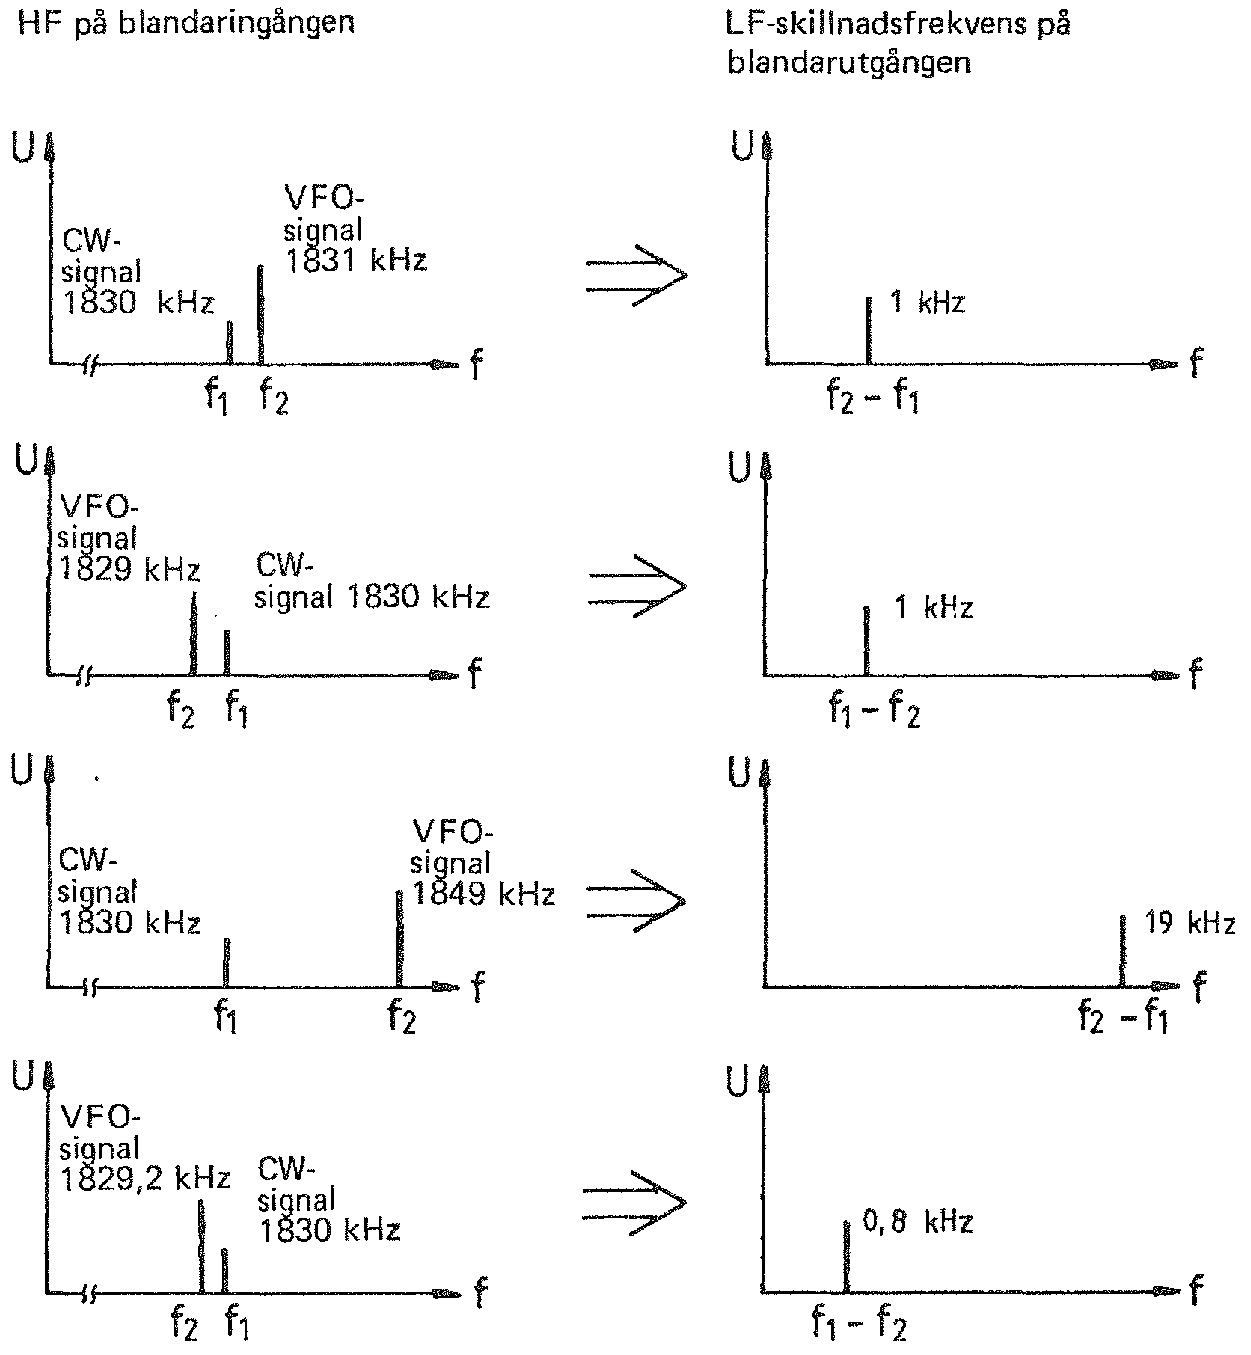
\includegraphics[width=\textwidth]{images/bild_2_4-09}
  \caption{Demodulering i mottagare med direkt frekvensomvandling- C W-signaler}
  \label{fig:bildII4-9}
\end{figure}

\begin{figure}
  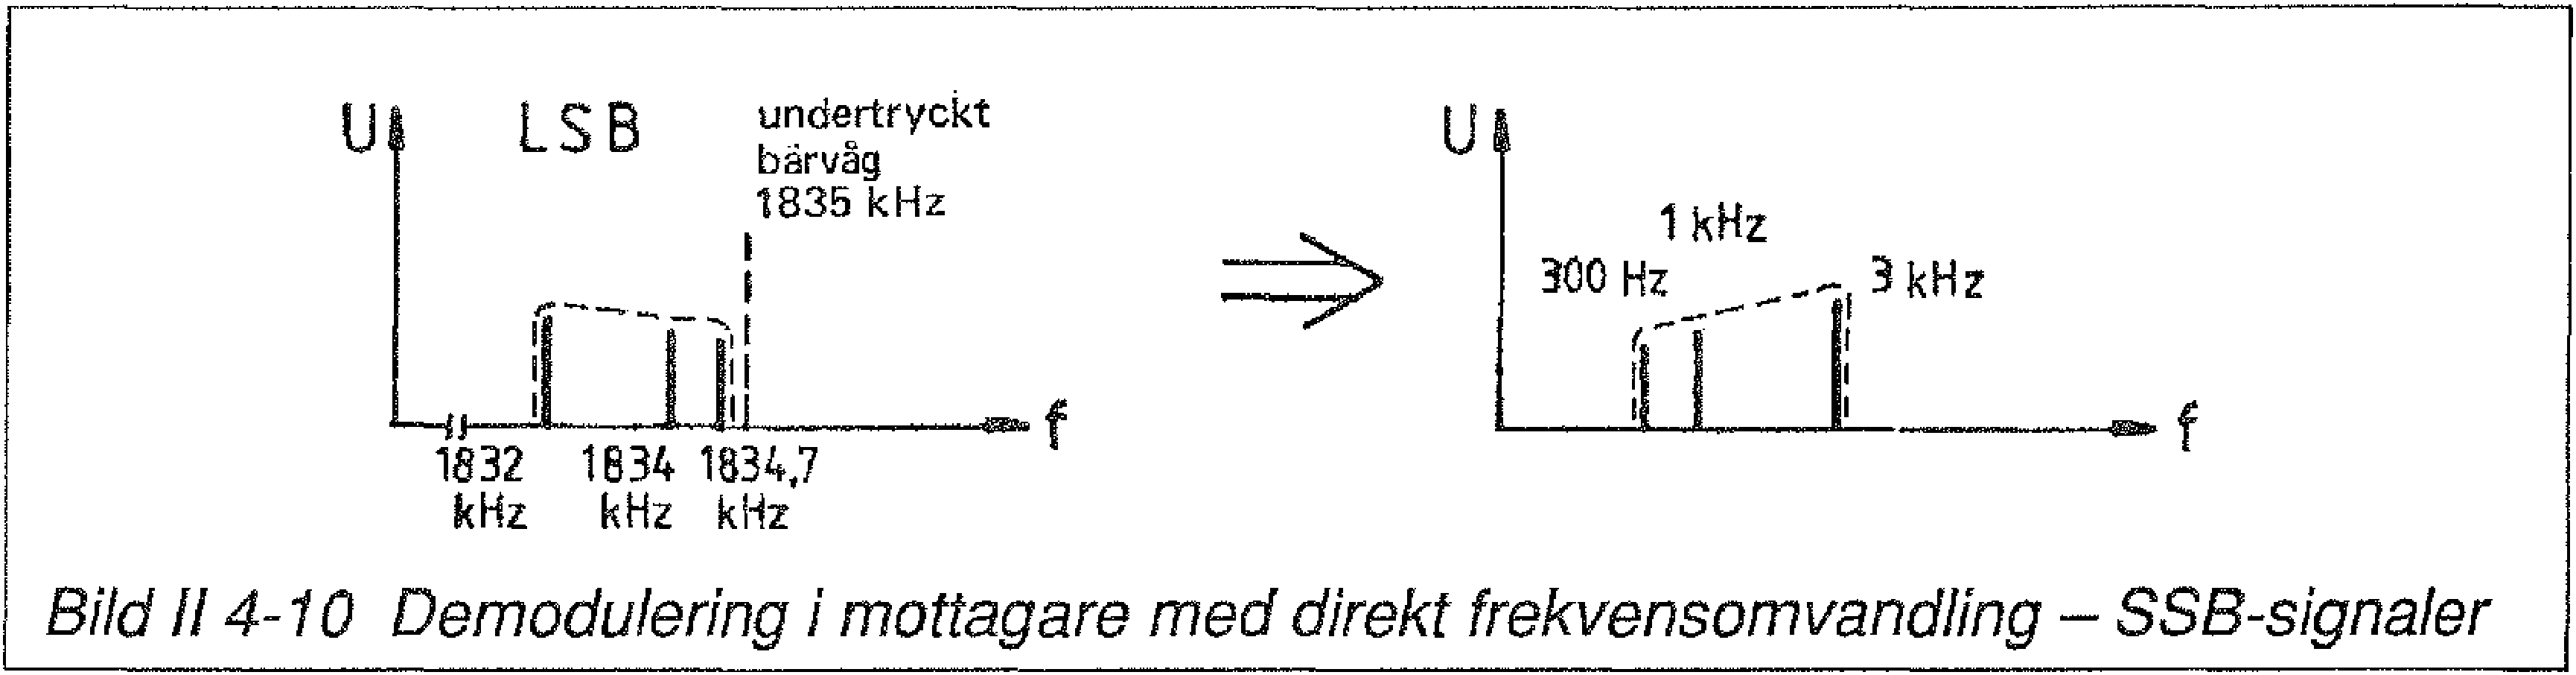
\includegraphics[width=\textwidth]{images/bild_2_4-10}
  \caption{Demodulering i mottagare med direkt frekvensomvandling - SSB-signaler}
  \label{fig:bildII4-10}
\end{figure}

\subsubsection{Mottagning av telegrafi (CW)}
\textbf{HAREC a.\ref{HAREC.a.4.2.1}\label{myHAREC.a.4.2.1}}
\index{CW}
\index{telegrafi}
\index{mottagare!CW}

Bild \ref{fig:bildII4-9}

Då BFO (VFO) är inställd på frekvensen \(f_2\) = 1831~kHz och den
mottagna signalen \(f_1\) har frekvensen 1830~kHz så hörs en
svävningston med frekvensen 1000~Hz.

Samma resultat fås om BFO ställs in på frekvensen \(f_2\) = 1829
kHz. Med BFO på frekvensen \(f_2\) = 1830~kHz hörs ingenting av
signalen \(f_1\) = 1830~kHz från sändaren.  Frekvensskillnaden är noll
Hz.

De flesta föredrar en ton med frekvensen c:a 800~Hz för mottagning av
telegrafi. BFO-frekvensen skulle i så fall ställas in på 1830,8 eller
1829,2~kHz om \(f_1\) vore en telegrafisändning.

\begin{figure}
  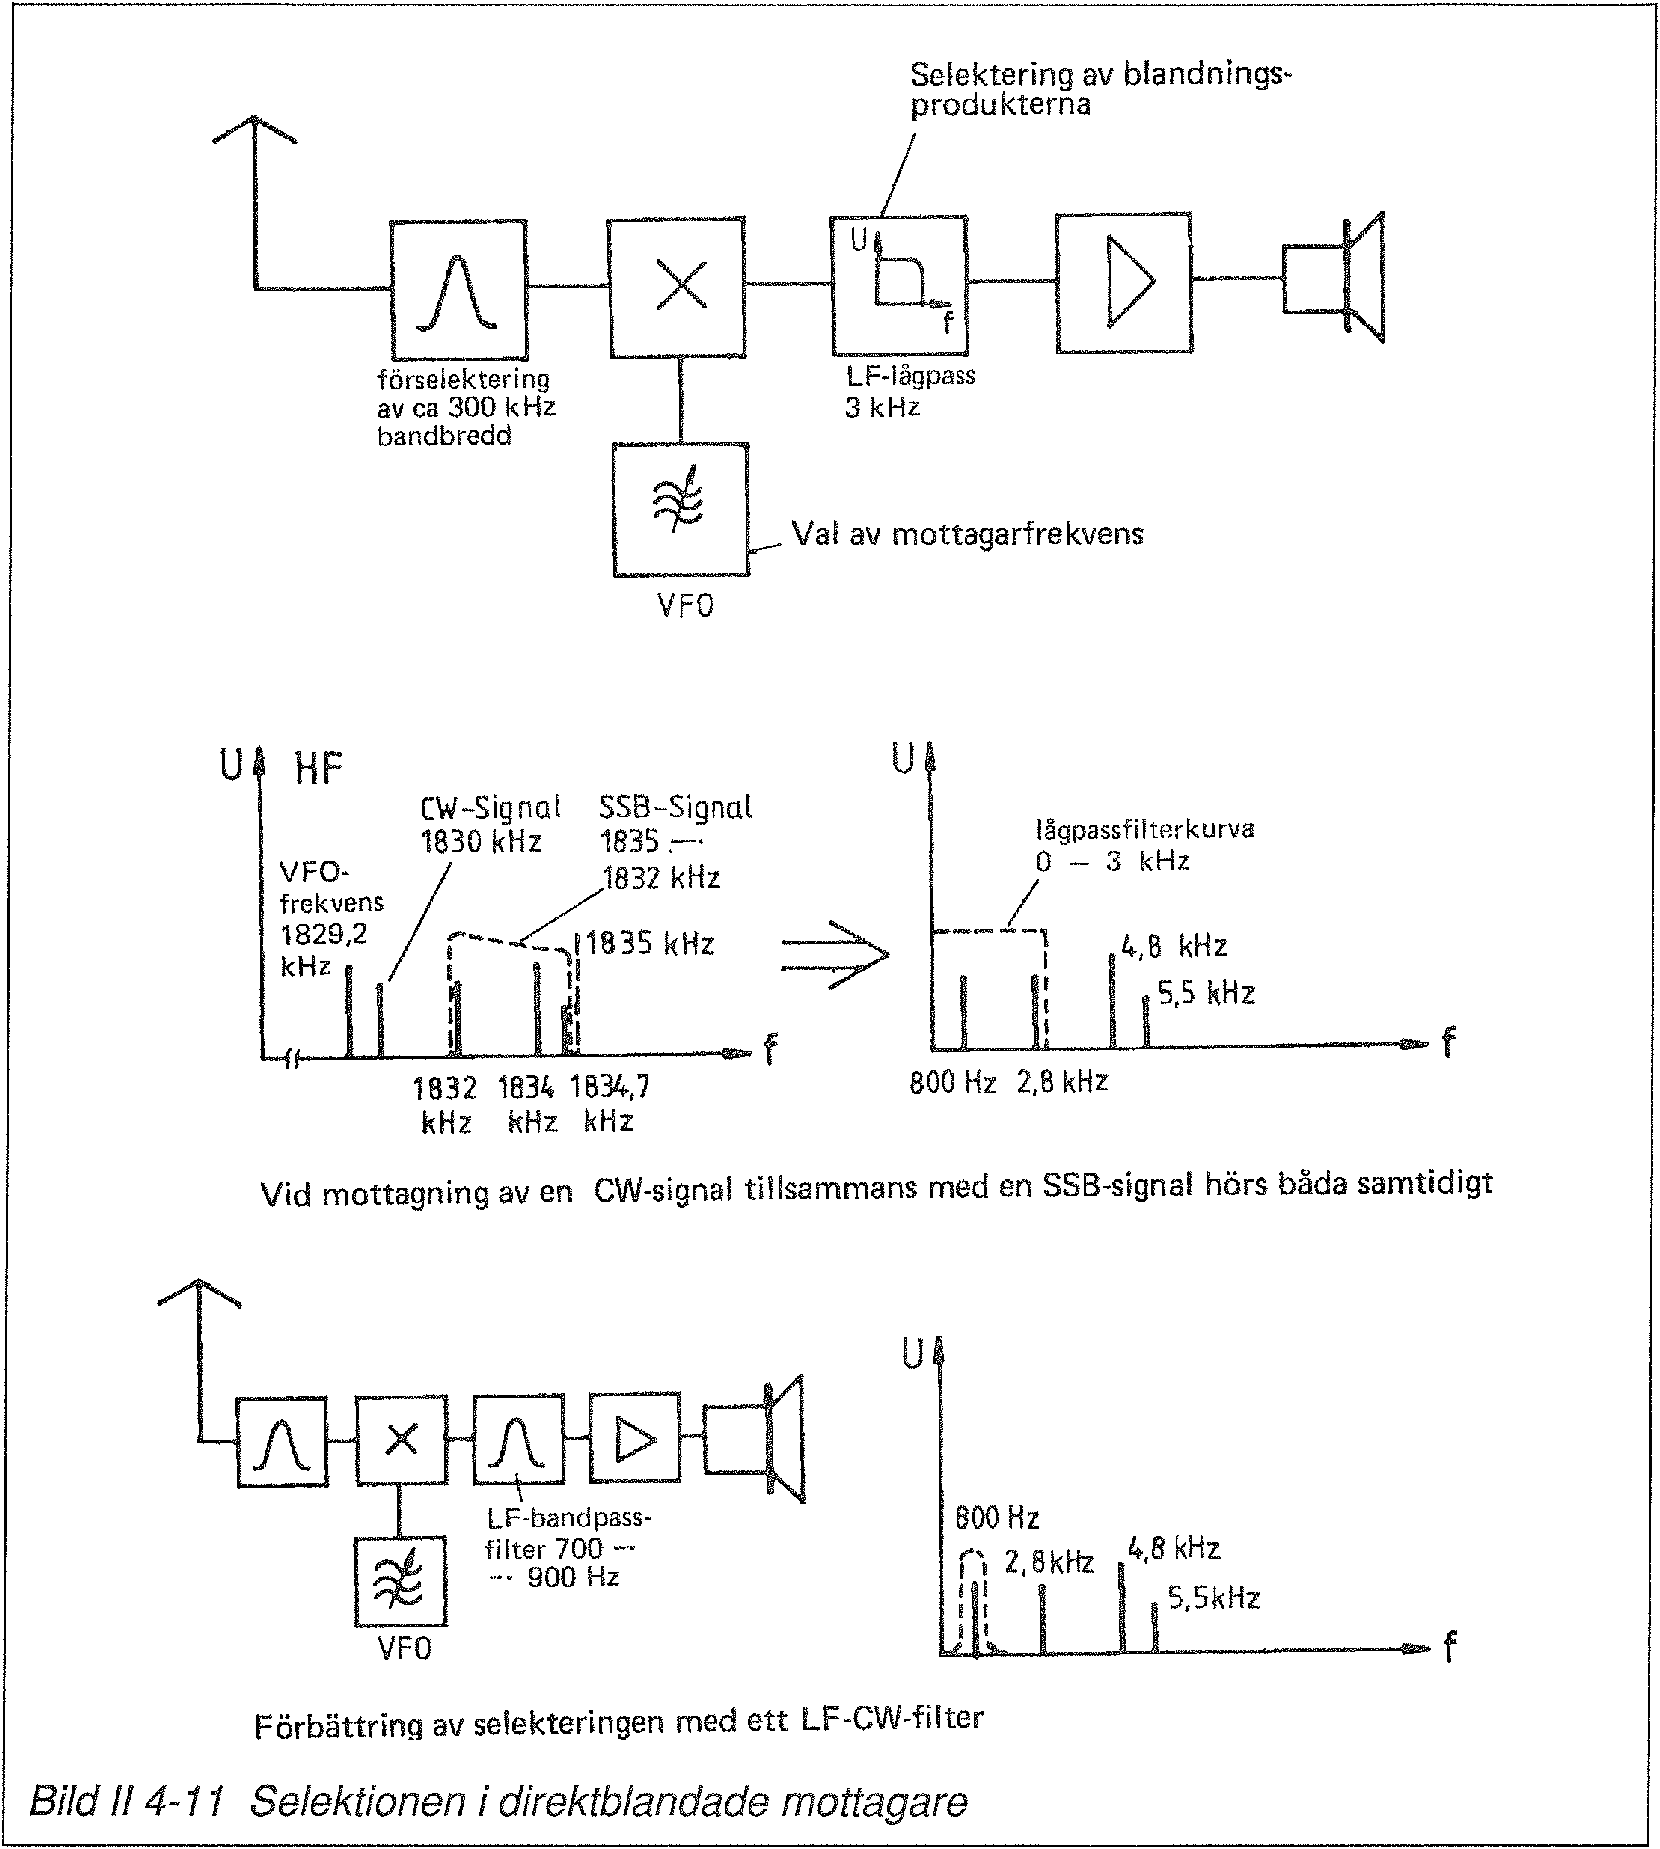
\includegraphics[width=\textwidth]{images/bild_2_4-11}
  \caption{Selektionen i direktblandade mottagare}
  \label{fig:bildII4-11}
\end{figure}

\subsubsection{Mottagning av J3E (SSB)}
\textbf{HAREC a.\ref{HAREC.a.4.2.3}\label{myHAREC.a.4.2.3}}
\index{J3E}
\index{SSB}
\index{mottagare!SSB}

När en SSB-sändare sägs arbeta t. ex. på frekvensen 1835~kHz, så
innebär det frekvensen på den bärvåg som undertryckts i sändaren redan
före utsändningen.

Vad som uppfattas av mottagarens ingångskretsar är alltså det utsända
sidbandet När en SSB-signal demoduleras, så blandas den lokala
bärvågen i mottagaren med de mottagna modulationsprodukterna.  Vid
blandningen uppstår blandningsprodukter som består dels av LF, dels av
andra högre frekvenser som dämpas i ett låg passfilter.

Bild \ref{fig:bildII4-10}

Inom amatörradio används för SSB det lägre sidbandet vid frekvenser
under 10~MHz.  Med en frekvens av t.ex. 1835~kHz och ett talspektrum
av 300-3000~Hz kommer det lägre sidbandet att finnas mellan 1834,7 och
1832,0~kHz. Tre modulerande frekvenser 300, 1000 och 3000~Hz visas på
bilden.

Med en bärvågsfrekvens av 1835~kHz motsvaras dessa modulerande
frekvenser av utfrekvenserna 1834.7, 1834 och 1832~kHz. VFO ersätter
SSB-sändarens bärvåg och ska ha samma frekvens - 1835~kHz - för att
kunna återge 300, 1000 och 3000~Hz.

\subsection{Selektionen i direktblandade mottagare}
\index{selektion}
\index{mottagare!selektion}

Bild \ref{fig:bildII4-11}

Direktblandade mottagare kan ses som en typ av detektormottagare, även
kallad ''rak'' mottagare. Begreppet ''rak'' kommer av att HF-signalen från
antennen passerar genom en selektiv krets och en eventuell
HF-förstärkare rakt fram till detektorn, utan att frekvensen omvandlas.

I en detektormottagare är bandbredden oftast rätt stor. Flera sändare
hörs därför samtidigt.

P.g.a. att blandningsdioden i en direktblandad mottagare även fungerar
som AM-demodulator, så hörs faktiskt alla sändare inom förkretsens
bandbredd. Detta kan undvikas till en del genom att dioden, som
fungerar som entaktsblandare, byts till en mottaktsblandare eller ännu
hellre till en ringblandare. Sådana blandare undertrycker
ingångsfrekvenserna och släpper endast igenom
blandningsprodukter. Bara den sändarsignal hörs då, vars frekvens
tillsammans med VFO-frekvensen ger blandningsprodukter, som faller
inom LF-filtrets passband. Mottagningsfrekvensen är
VFO-frekvensen. Svängningskretsen fungerar som en ställbar förselektor
och LF-lågpassfiltret ger den egentliga frekvensselektionen.

Vilka HF-signaler bildar blandningsprodukter med VFO-frekvensen och
vilka av dessa passerar sedan genom lågpassfiltret efter nedblandning
till LF-nivå?

Exempel: En CW-sändare med frekvensen 1830~kHz tas emot genom att
mottagarens VFO ställs in på frekvensen 1829,2~kHz. Från
blandarutgången kommer då en ton med frekvensen 800~Hz.

Men sändaren är inte ensam på bandet.  Kommer t.ex. SSB-sändaren på
1835, som moduleras med 300, 1000 och 3000~Hz, att störa mottagningen?
(Bild \ref{fig:bildII4-10}).

Förkretsen i mottagaren är så bred att denna sändning
passerar. SSB-sändarens signalfrekvenser i det utsända sidbandet är
1834,7, 1834,0 och 1832~kHz. Dessa frekvenser blandas med mottagarens
VFO-frekvens 1829,2~kHz och alstrar blandningsprodukterna 5,5, 4,8 och
2,8~kHz. Eftersom lågpassfiltret i mottagarens LF-förstärkare har
bandbredden 0-3000~Hz, så kommer endast blandningsprodukten 2,8~kHz
att vara störande. För att förbättra CW-mottagningen, så kan
lågpassfiltret bytas ut mot ett bandpassfilter, som endast släpper
igenom ett smalt frekvensområde omkring mittfrekvensen 800~Hz.

\subsection{Passband och spegelfrekvenser i direktblandare}
\index{passband}
\index{spegelfrekvenser}
\index{direktblandare}
\index{blandare!spegelfrekvenser}

Bild \ref{fig:bildII4-12}

I exemplet i förra stycket blev problemet med en störande ton löst med
ett bandpassfilter med annan frekvensgång.  Men vilka frekvenser kan
tas emot genom ett lågpassfilter, 0--3000~Hz, om VFO-frekvensen är
t.ex. 1829,2~kHz?


Experiment: Ändra frekvensen på en CW-sändare långsamt från 1820 till
1840~kHz.

Sändarfrekvensen 1820~kHz hörs knappast eftersom överlagringstonen har
frekvensen 9,2~kHz och den dämpas kraftigt av lågpassfiltret. Först
när sändarfrekvensen är 1826,2~kHz hörs en tydlig ton med frekvensen
3000~Hz. Fortsätter man att ändra sändarfrekvensen, så sjunker tonens
frekvens för att bli noll (svävningsnoll), när sändarfrekvensen är
lika med mottagarens VFO-frekvens 1829,2~kHz. Om man nu fortsätter med
att höja frekvens, så blir överlagringstonens frekvens åter högre. Vid
sändarfrekvensen 1832,2 är den 3000~Hz. Vid ännu högre sändarfrekvens
dämpas överlagringstonen igen av lågpassfiltret

Slutsatsen av experimentet blir följande: Vid en direktblandande
mottagare med VFO-frekvensen 1829,2~kHz och ett 3~kHz lågpassfilter
blir varje sändare hörbar, som har en sändningsfrekvens mellan 1826,2
och 1832,2, varvid överlagringstonen har frekvenser från 3000~Hz, ner
genom noll och upp till 3000~Hz igen.

\begin{figure}
  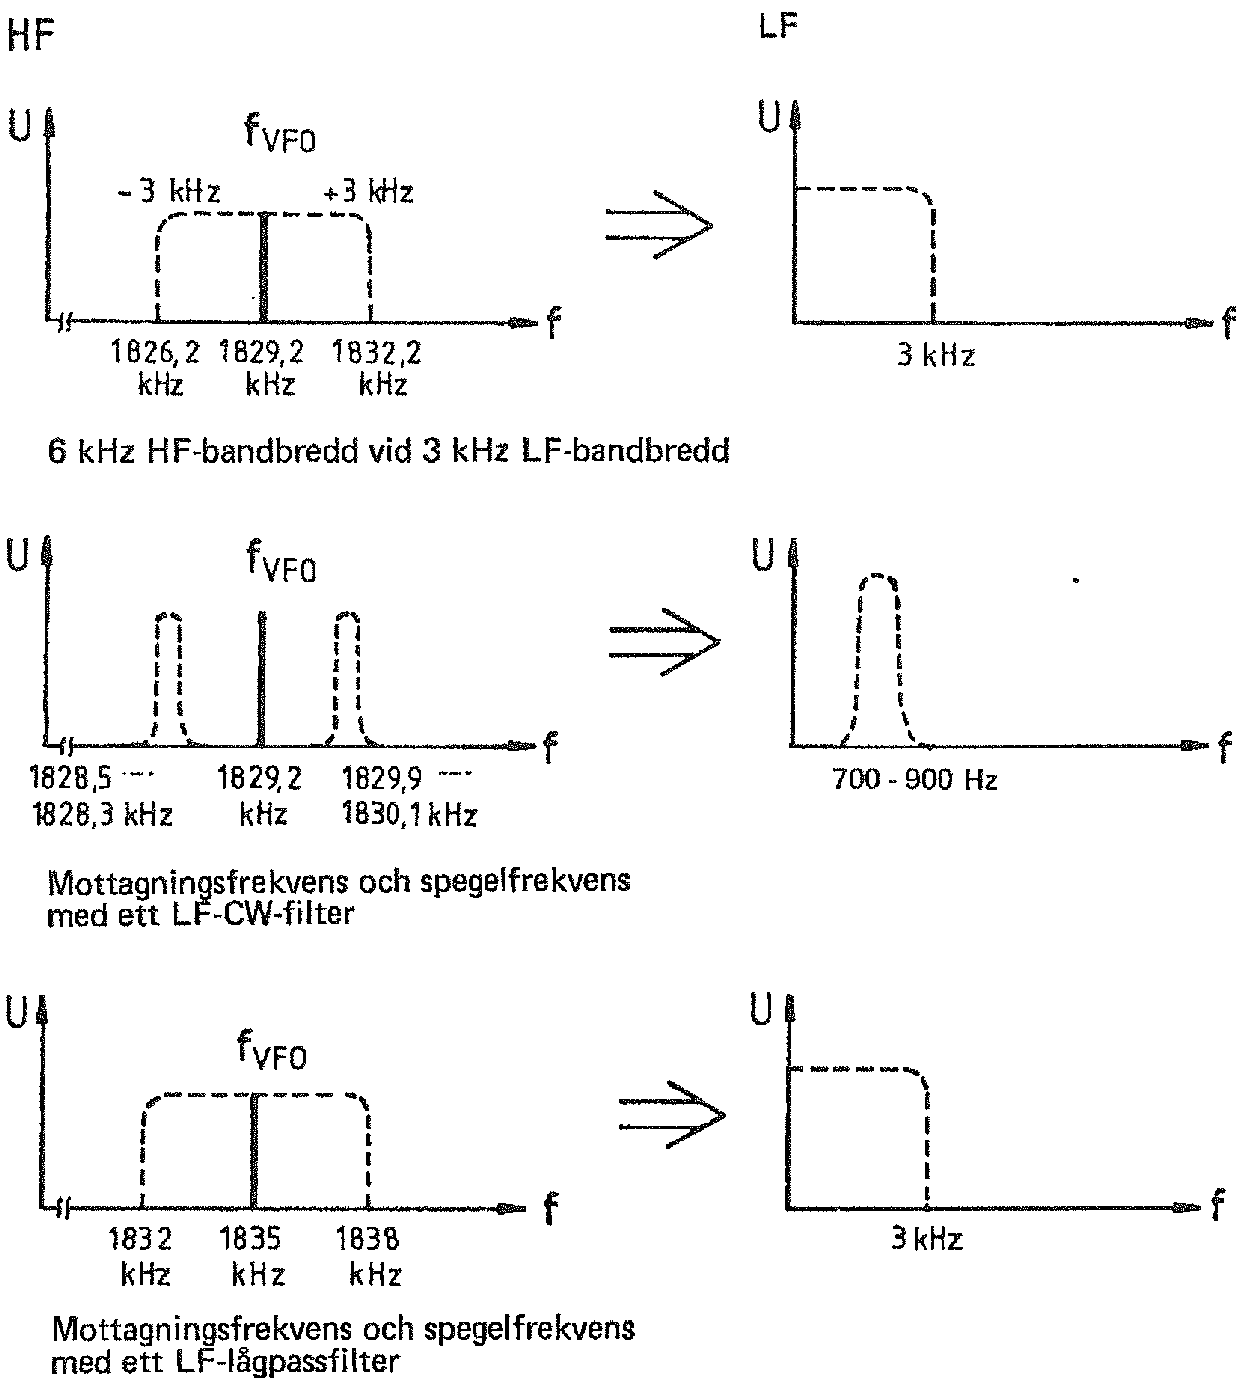
\includegraphics[width=\textwidth]{images/bild_2_4-12}
  \caption{Passbandbredd och spegelfrekvenser i direktblandade mottagare}
  \label{fig:bildII4-12}
\end{figure}

Vår mottagare har bandbredden 6~kHz.  Varje annan sändare inom denna
passbandbredd kommer att höras eller - om man så tycker - störa
mottagningen.

Tillbaka till exemplet med bandpassfiltret. Vilka frekvenser kan tas
emot med ett bandpassfilter 700-900~Hz (mittfrekvens 800~Hz), om
VFO-frekvensen är 1829,2~kHz?  Jo, vi kan lyssna rätt ostört till vår
CW-sändares 800~Hz-ton på frekvensen 1830~kHz. Ändå kan en annan
sändare med frekvensen 1828,4~kHz störa mottagningen därför att denna
är spegelfrekvens till mottagningsfrekvensen 1830~kHz. Vid
VFO-frekvensen 1829,2~kHz uppstår en överlagringston, inte bara vid
sändarfrekvensen 1830~kHz utan också vid 1828,2~kHz. Även denna andra
sändarfrekvens, liksom nyttofrekvensen, släpps igenom bandpassfiltret

Spegelfrekvensmottagning är en principiell nackdel i mottagare med
direktblandning. Nyttofrekvens och spegelfrekvens i det senaste
exemplet ligger 1,6~kHz (\(2 \cdot 800\) Hz) ifrån varandra, alltså
dubbla värdet av bandpassfiltrets mittfrekvens.

Vid SSB-mottagning måste naturligtvis hela LF-området upp till 3000~Hz
kunna släppas igenom. Utöver det önskade frekvensområdet 1832-1835
kHz, kommer även spegelfrekvenser i området 1835-1838~kHz att kunna
tas emot.

Vid en LF-bandbredd av 3~kHz har således den direktblandade mottagaren
en bandbredd av 6~kHz, vilket är en god avstämningsskärpa i jämförelse
med den 300~kHz breda förkretsen.

\subsection{För- och nackdelar med direktblandare}

Enkel uppbyggnad, men trots det en god känslighet och hygglig
avstämningsskärpa.  VFO kan även användas till att styra en sändare.

Spegelfrekvensmottagning är tyvärr oundviklig. Vidare kan signaler
från starka sändare stråla in i den känsliga LF-förstärkaren och
orsaka LF-detektering, om mottagaren är otillräckligt
skärmad. Förbättrad isolering mellan antenn och VFO kan dock fås med
en HF-förstärkare.

Entakts diodblandare är olämplig i en direktblandad mottagare. Den tar
emot alla sändare inom förkretsens passband och en del av VFO-signalen
kommer att strålas ut i antennen. Ingen av dessa nackdelar finns i en
mottakts- eller ringblandare.
